\documentclass[article, 11pt]{IEEEtran}   %Document is an article, 11 pt font, and follows IEEE format

%Aqui van todos los paquetes que van a utilizar para el documento
\usepackage{hyperref}         %Uso paquete hyperref  (hiperlinks)
\usepackage{graphicx}         %Uso paquete  graphicx  (imágenes)
\usepackage{float}            %Uso paquete  float  (posicionar imágenes)
\usepackage{gensymb}          %Uso paquete  gensymb  (simbolos)
\usepackage{amsmath}          %Uso paquete  amsmath  (formulas matemáticas)
\usepackage{tikz}             %Uso paquete  tikz  (crear gráficas)
\usepackage{pgfplots}         %Uso paquete  pgfplots  (crear gráficas)
\usepackage{pgfplotstable}    %Uso paquete  pgfplotstable (regresión lineal)
\usepackage[spanish]{babel}	  %Uso paquete  babel spanish (caracteres en español)
\usepackage{lipsum}  		  %Uso paquete  lipsum (crea dummy text)

\begin{document}

%TITULO DEL REPORTE
%Las palabras inician con mayúscula excepto las preposiciones
\title{Final Project\\ Modelation and Simulation of Systems - Rocket}


%INFORMACIÓN DEL AUTOR O AUTORES
\author{\IEEEauthorblockN{José Barreno\\Luis Guzmán\\Byron García\\José Rivera}
\IEEEauthorblockA{\\Universidad Galileo, Systems Theory II\\Guatemala, Guatemala}}


% make the title area
\maketitle



%Resumen
%Esta sección es un breve resumen de los aspectos más importantes del proyecto. Se incluye el objetivo del proyecto, los hallazgos más importantes y la conclusión principal.

\begin{abstract}
\lipsum[1-1]
\end{abstract}


%INTRODUCCIÓN
%Esta sección incluye el objetivo del proyecto. Se deben incluir los %siguientes temas:
% Contexto de aprendizaje -> de que trata el proyecto, incluir el background teorico, incluir las referencias!
%El proposito del proyecto -> se incluye la hipótesis que desea probar, o la serie de preguntas que se desean contestar
%Breve resumen de la metodología utilizada y de los resultados que esperan obtener

%Link de ayuda: https://libguides.usc.edu/writingguide/introduction
\section{Introducci\'on}
\begin{otherlanguage}{english}
\section{Introduction}
When a rocket is launching, you have to control its forward acceleration and the direction it's pointing at the same time. The tricky part is that these two are highly coupled. If the thrust is slightly misaligned, it creates a pitching moment; if the pitch changes, it messes with the axial acceleration. Because of this, we can't just treat thrust and attitude as separate SISO (single-input, single-output) systems—if we do, we'll miss the crosstalk that can tank our tracking performance or make the rocket unstable. To study this, the project uses a simplified MIMO (multiple-input, multiple-output) model of a rocket moving just in the pitch plane.

To keep the math manageable, we linearized the model around a specific point during ascent. For this specific window, we're assuming small angles, constant mass and inertia, and steady aerodynamic conditions. The system has four main states: axial acceleration, pitch angle, pitch angular velocity, and nozzle deflection. We feed it acceleration and pitch commands, and measure the actual acceleration and pitch angle as outputs. The model also factors in the engine and nozzle-servo dynamics, aero damping, that destabilizing aerodynamic stiffness, and IMU feedback. The $K_1$ and $K_2$ gains are already baked into the governing equations to set the strength of the thrust and direction feedback loops.

The main goal here is to connect the math of the system back to what the rocket is actually doing physically. We're hitting it with a mix of state-space and transfer matrices, plus running stability checks, time-domain sims, frequency response, and the usual controllability and observability tests. We're mainly looking at how tweaking the control gains changes response speed, oscillations, and the interaction between the two outputs. In the frequency domain, we're checking the four input-output paths to find their bandwidths and resonance, and to see if we can actually get away with treating them as independent channels. All of this basically sets us up to pick the right gains and figure out the real-world implications of running this controller with a finite sampling time.

\end{otherlanguage}


%METODOLOGÍA
%Incluye todos los pasos que se deben seguir para llevar a cabo el experimento. Además debe incluir la justificación de la aplicación de los procedimientos. Se debe incluir cómo se obtuvo la data, qué tipo de data es y cómo fue analizada.
\section{Metodolog\'ia}
\lipsum[1-2]

%RESULTADOS
%Incluye únicamente todos los resultados obtenidos del experimentos. Pueden ser presentados en forma de tabla o gráficas. Incluye pequeños parrafos en donde es explique qué es lo que se esta presentando, o a que resultado poner atención. Sin embargo, no incluyen la interpretación de estos.
\section {Resultados}
After an analisys of the system, we found that the system models the atmosferic ascen of a rocket in the logitudinal axis, so the system start in the bloque one that has the entries of u1 and u2, for the axial aceleration and the pitch angle, those entries are passed to the central computer after pass of a converted from analog to digital to can analyse where the rocket is possioned to start making the adjustments

\subsection{Seccion A.1}
El modelo describe el movimiento de un cohete a través de un eje longitudinal que es controlado por una aceleración axial y un angulo de cabeceo para ajustar su dirección, el sistema procesa la información a través de la computadora de abordo después de haber pasado por una conversión de valores análogos a digitales para poder hacer los cálculos computacionales, reflejado en los bloques 1,2 y 3 de la figura 1, en donde se hacen los ajustes necesarios para asegurar la integridad del cohete y la trayectoria deseada, luego en los bloques 4 y 5 se envían los ajustes a través del amplificador para corregir la deflexión de la tobera lo que generara algo de inestabilidad que es registrada en el bloque 6 según que considera la dinámica del cohete, una vez obtenido estos datos, el acelerómetro y la IMU realizan sus lecturas para enviar la retroalimentación al bloque 3 que volverá a ajustar los valores hasta lograr una estabilidad esto debido a que el sistema tiene acoplamiento, y cualquier intento por corregir la aceleración o el angulo de cabeceo genera inestabilidad, el sistema maneja varios parámetros empezando por las entradas u1 y u2 que son los comandos inicales de ajuste deseados convertidos a un muestreo digital para que la computadora pueda realizar sus cálculos por el periodo de ese muestreo, en este proceso entran los valores de ganacia K1 y K2 que son los que ayudan a definir la medida o magnitud de cambios que se aplicarían a los comandos de ajustes, cada calculo esta también afectado por los parámetros adicionales que modela el sistema integrados en las ecuaciones de estado,
\begin{itemize}
\item k\_a: Es el factor de conversión entre la señal enviada por el amplificador y el empuje netodel motor.
\item tau\_m: Es la velocidad de respuesta de la propulsión, el retraso con el que actua el motor luego del envio del ajuste.
\item c\_theta: Representa la perdida en la aceleragion generado por la gravedad en el eje axial del cohete.
\item Mu: Representa el momento aerodinámico generado cuando el Centro de Presión (CP) está por delante del Centro de Masa (CM). La fuerza de torcion resultante al aplicar cualquer angulo de ajuste mayor a 0, lo que genera la inestabilidad.
\item a\_d: Representa el momento de fricción que ejerce el aire contra el fuselaje al rotar, oponiéndose a la velocidad angular, este tambien influye en la desestabilizar el cohete.
\item k\_delta: Es el empuje vectorial que genera torque, para controlar el angulo de ajuste para la tobera.
\item k\_epsilon: Torque parásito generado por el ajuste en el angulo de cabeceo que, dado la aplicación de una aceleracion axial desaliniada al CM.
\item tau\_s: Representa el tiempo de reaccion de para corregir el angulo de la tobera el cual es significativamente mas pequeño que tau\_m para evital que se apliquen aceleraciones o empuge en angulos incorrectos que pueden peligrosos.
\item Lambda: representa una realacion velocidad-posicion en la retroalimentación, que ayuda a justar los calculos para ayudar a reducir oscilaciones dado los ajustes acoplados.
\item T: Es el intervalo de tiempo entre los ciclos de la computadora a bordo, el cual debe ser lo suficientemente rapido para lograr analizar los datos cambiantes en el tiempo.
\end{itemize}
En todo este flujo del sistema, hay que hacer especial énfasis en los valores K1 y K2 dado que esos valores nos ayudan a mejorar la respuesta del sistema antes los ajustes deseados, con un valora mayor de K1, el ajuste en el valor de empuje o aceleración se alcance con mayor rapidez lo que ayuda a evitar osculaciones e inestabilidad, lo mismo para K2, que es la rapidez con la que el sistema mecanico actual para ajustar la tobera y cambiar la defleccion que este genera y generar la suficiente fuerza para ajustar la tobera, sin embargo hay que considerar que este no tiene que susperar la respuesta física de los sistemas que controlan mecánicamente el ajuste porque el sistema podría fallar, (pendiente de definir un rango de eficiencia de K1 y K2)

\subsection{Seccion A.2}
A continuación se presenta el diagrama de simulación del sistema, reemplazando algunos parámetros con variables simbólicas $g_i$ para simplificar el diagrama, cuya traducción esta en la tabla 1
$$x_1 = a(t)$$
$$x_2 = \theta(t)$$
$$x_3 = \omega(t)$$
$$x_4 = \delta(t)$$

Here is the simulation diagram:

\begin{figure}[H]
\centering
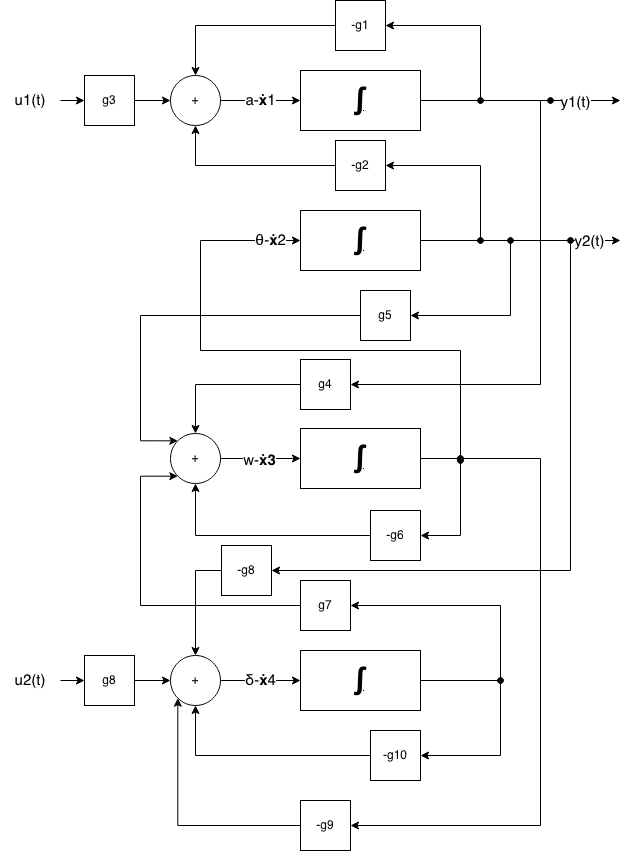
\includegraphics[width=\columnwidth]{imgs/TSII - Simulation Diagram.drawio.png}
\caption{Simulation diagram of the rocket system.}
\label{fig:simdiagram}
\end{figure}

\begin{table}[H]
\centering
\caption{Traducción de símbolos}
\begin{tabular}{|c|c|}
\hline
Símbolo & Valor \\
\hline
$g_1$ & $(1 + K_1 k_a)/\tau_m$ \\
$g_2$ & $c_\theta$ \\
$g_3$ & $K_1 k_a/\tau_m$ \\
$g_4$ & $k_\epsilon$ \\
$g_5$ & $\mu$ \\
$g_6$ & $a_d$ \\
$g_7$ & $k_\delta$ \\
$g_{10}$ & $1/\tau_s$ \\
$g_8$ & $K_2/\tau_s$ \\
$g_9$ & $\lambda K_2/\tau_s$ \\
\hline
\end{tabular}
\end{table}

pendiente de generar análisis de trayectorias y valires de K1

\subsection{Seccion A3}
Vector de estados y de entradas:
\begin{equation*}
\mathbf{x}(t)=\begin{bmatrix}x_1\\x_2\\x_3\\x_4\end{bmatrix}=\begin{bmatrix}a(t)\\\theta(t)\\\omega(t)\\\delta(t)\end{bmatrix},\qquad
\mathbf{u}(t)=\begin{bmatrix}u_1(t)\\u_2(t)\end{bmatrix}
\end{equation*}

Ecuaci\'on de estados $\dot{\mathbf{x}}(t)=A\mathbf{x}(t)+B\mathbf{u}(t)$:
\begin{equation*}
\resizebox{\columnwidth}{!}{$
\begin{bmatrix}\dot a\\\dot\theta\\\dot\omega\\\dot\delta\end{bmatrix}=
\begin{bmatrix}
-\frac{1+K_1k_a}{\tau_m} & -c_\theta & 0 & 0\\
0 & 0 & 1 & 0\\
k_\epsilon & \mu & -a_d & k_\delta\\
0 & -\frac{K_2}{\tau_s} & -\frac{\lambda K_2}{\tau_s} & -\frac{1}{\tau_s}
\end{bmatrix}
\begin{bmatrix}a\\\theta\\\omega\\\delta\end{bmatrix}+
\begin{bmatrix}
\frac{K_1k_a}{\tau_m} & 0\\
0 & 0\\
0 & 0\\
0 & \frac{K_2}{\tau_s}
\end{bmatrix}
\begin{bmatrix}u_1\\u_2\end{bmatrix}
$}
\end{equation*}

\subsection{Seccion A4}
\begin{equation*}
G_{ij}(p)=\frac{N_{ij}(p;K_1,K_2)}{D(p;K_1,K_2)},\qquad D(p)=\det(pI-A)
\end{equation*}

\begin{align*}
D(p)&=p^4+p^3(0.069902K_1+21.417)\\
&\quad+p^2(1.4225K_1+102.0K_2+27.518)\\
&\quad+p(7.13K_1K_2+0.40543K_1+278.85K_2-16.633)\\
&\quad+11.883K_1K_2-1.6776K_1+181.42K_2-2.0688\\
N_{11}(p)&=0.0034951K_1(2040.0K_2p+3400.0K_2\\
&\quad+20.0p^3+407.0p^2+116.0p-480.0)\\
N_{12}(p)&=-1667.7K_2\\
N_{21}(p)&=0.0083882K_1(p+20.0)\\
N_{22}(p)&=0.000136K_2(87377.0K_1+1.25\cdot10^{6}p+1.334\cdot10^{6})
\end{align*}

Para $K_1=1,\ K_2=0.5$:
\begin{equation*}
D(p)=p^4+21.487p^3+79.94p^2+126.76p+92.907
\end{equation*}


\subsection{Tabla de datos}
\begin{table}[H]
\centering
\caption{Ejemplo de Tabla con datos}
\label{DataTable1}
\begin{tabular}{|c|c|}
\hline
X [s] & Y[m/s]  \\
\hline
11.7 & 37.8              \\
17.1 & 54     \\  
8.4 & 26.6 \\
6.6 & 21.2 \\
7.4 & 23.4 \\
1.9 & 7   \\
\hline   
\end{tabular}
\end{table}

%EJEMPLO DE COMO UTILIZAR LOS PAQUETES PARA CREAR UNA GRAFICA
\subsection{Gr\'aficas}
\begin{figure}[H]
	\centering
	\begin{tikzpicture}
		\begin{axis}[
   			title=Puntos obtenidos,	%Title of graph
   			xlabel={x[s]},			%label the x-axis
  			ylabel={y[m/s]},		%label the y-axis
   			legend pos=south east,	%put slope legend in bottom right corner
]
			\addplot[blue, only marks] table[col sep=comma] {data/CircleData.csv};	%plot points from data table
			\addplot [red] table[col sep=comma, y={create col/linear regression={y=y}}]   %best fit line
        {data/CircleData.csv};
       
			\addlegendentry{slope=$\pgfmathprintnumber{\pgfplotstableregressiona}$}        
        %show slope value
		\end{axis}
	\end{tikzpicture}
	\caption{Ejemplo de gr\'afica}\label{diagram1}   %caption the graph
\end{figure}


%==========================================================================
% Partes D y E. Siguen el contenido y el orden de Reporte_explicado_ES.pdf
% (idea, ubicación en el notebook, lectura de gráficas e implicaciones),
% redactados como texto continuo. Los cálculos completos están en
% TSII-PROJECT-NB.ipynb (celdas 77 a 89).
%==========================================================================
\subsection{Secci\'on D.11: observabilidad}

La computadora de a bordo solo cuenta con dos sensores, el acelerómetro ($a$) y la IMU ($\theta$), pero para corregir bien necesita conocer los cuatro estados, incluyendo la velocidad angular $\omega$ y la deflexión de la tobera $\delta$, que no se miden. La pregunta, entonces, es si esas dos variables pueden deducirse a partir de las mediciones; cuando esto es posible, se dice que el sistema es \emph{observable}. Para verificarlo se calcula la matriz de observabilidad $\mathcal{O}=[C;\,CA;\,CA^2;\,CA^3]$, que debe tener rango 4. Además, su valor singular más pequeño, $\sigma_{\min}(\mathcal{O})$, indica qué tan bien se observa: un valor cercano a cero significa que el sistema es ``observable en teoría, pero muy ruidoso en la práctica''. Estos cálculos se encuentran en la celda 77 del notebook (función \texttt{check\_system\_properties}), que incluye además dos casos de prueba que rompen la observabilidad a propósito.

Los resultados de la Tabla~\ref{tab:obs} muestran que, con ambos sensores, el rango es 4 y $\sigma_{\min}=1.17$, es decir, el cohete se observa muy bien. Con solo el acelerómetro el resultado es casi igual, ya que al inclinarse el cohete cambia la componente de la gravedad sobre su eje y, por lo tanto, el acelerómetro ``siente'' el cabeceo. En cambio, con solo la IMU el rango sigue siendo 4, pero $\sigma_{\min}$ cae a 0.026: el sistema es observable, aunque poco confiable, porque el ángulo solo se entera del empuje a través de la pequeña desalineación $k_\varepsilon$. Los dos casos de prueba refuerzan esta lectura, pues al anular esos acoplamientos ($c_\theta=0$ o $k_\varepsilon=0$) el rango cae a 1 y a 3, y el sistema deja de ser observable. En otras palabras, el mismo \emph{acoplamiento} que complica el control es el que permite deducir los estados que no se miden.

\begin{table}[H]
\centering
\caption{Observabilidad ($K_1=1$, $K_2=0.5$)}
\label{tab:obs}
\begin{tabular}{|l|c|c|}
\hline
Sensores & rango $\mathcal{O}$ & $\sigma_{\min}(\mathcal{O})$\\
\hline
$a$ y $\theta$ & 4 & 1.17\\
solo $a$ & 4 & 0.99\\
solo $\theta$ & 4 & 0.026\\
solo $a$, con $c_\theta=0$ & 1 & 0\\
solo $\theta$, con $k_\varepsilon=0$ & 3 & 0\\
\hline
\end{tabular}
\end{table}

Para comprobarlo en simulación, en la celda 79 se construyó un observador de Luenberger con \texttt{place\_poles}. Un observador funciona como un ``simulador en paralelo'': es una copia del modelo que corre en la computadora y se corrige continuamente con las mediciones. La Fig.~\ref{fig:obs} grafica juntos el valor real y el estimado, de modo que se ve de inmediato si el segundo alcanza al primero. Partiendo de cero, el estimado se pega al real en menos de 3~s, con un error final del orden de $10^{-9}$. Con solo la IMU también converge, aunque a costa de ganancias enormes ($|L|\approx3740$, frente a 22.5 con solo el acelerómetro), que en la práctica amplificarían el ruido del sensor.

\begin{figure}[H]
\centering
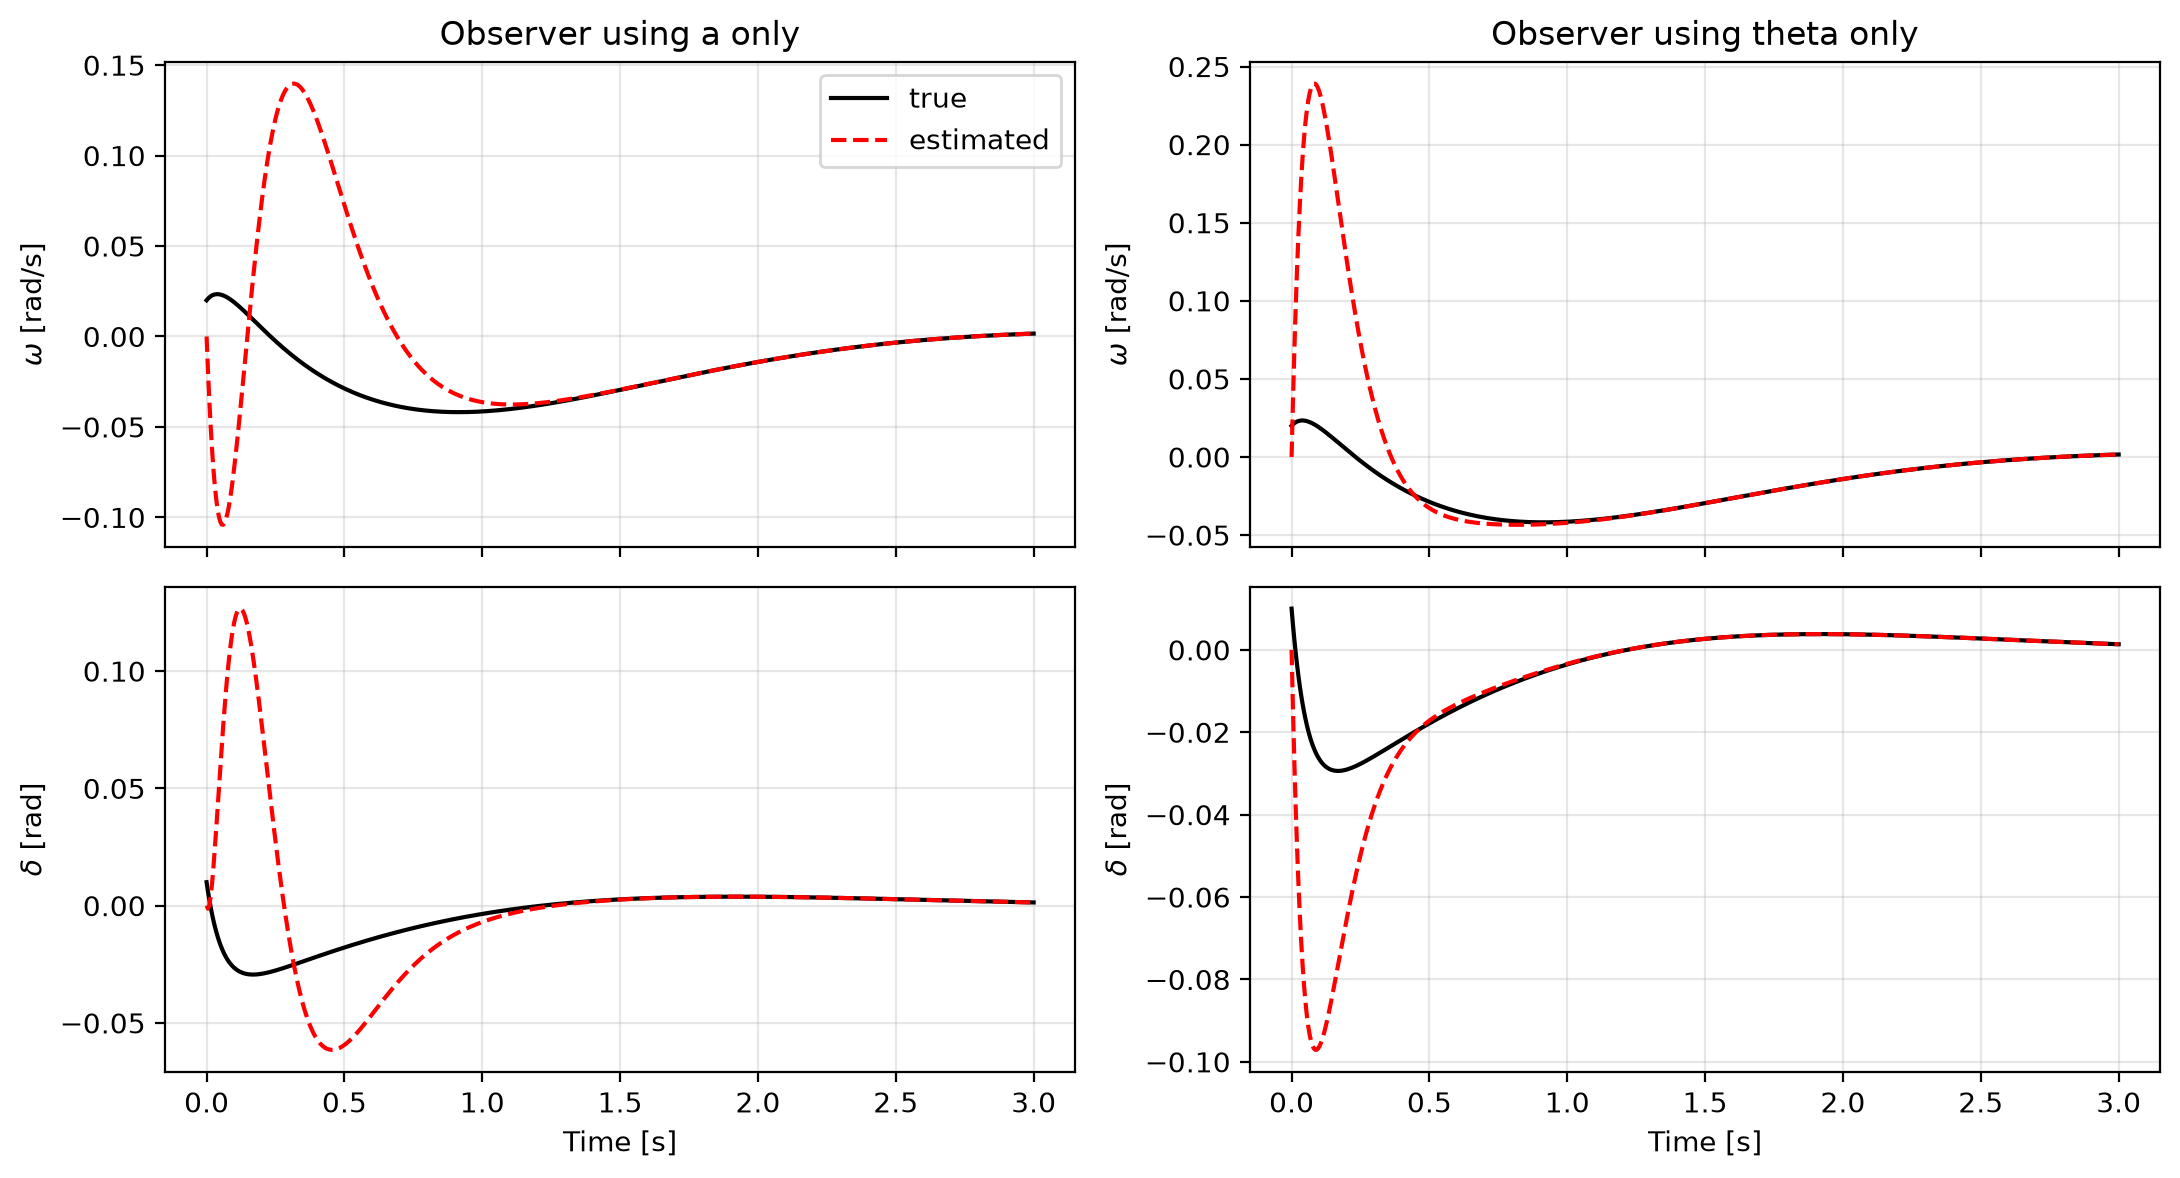
\includegraphics[width=\columnwidth]{imgs/fig_observer.png}
\caption{Observador que parte de cero: estimación de $\omega$ y $\delta$ usando solo el acelerómetro (izquierda) o solo la IMU (derecha). Negro: valor real; rojo discontinuo: estimado.}
\label{fig:obs}
\end{figure}

Por lo tanto, sí es posible reconstruir $\omega$ y $\delta$ sin medirlas, preferiblemente apoyándose en el acelerómetro. Si el sistema no fuera observable, la situación sería muy distinta: habría un movimiento interno invisible para los sensores y, como el cohete es aerodinámicamente inestable, ese movimiento podría crecer sin ser detectado. La computadora corregiría entonces con un estado equivocado; por ejemplo, no notaría una tobera que se desvía o se traba hasta que el ángulo ya fuera grande.

\subsection{Secci\'on D.12: controlabilidad}

La controlabilidad plantea la pregunta inversa: si las entradas disponibles pueden llevar el sistema a cualquier estado. Para responderla se usa la matriz de controlabilidad $\mathcal{C}=[B,\ AB,\ A^2B,\ A^3B]$, que también debe tener rango 4, y se prueba qué ocurre cuando falla un actuador: el servo de la tobera se traba y solo queda $u_1$, falla el control de empuje y solo queda $u_2$, o se apaga la dirección ($K_2=0$). Este análisis está en la celda 81 del notebook, donde la función \texttt{controllability\_report} calcula para cada escenario el rango, $\sigma_{\min}$, los estados fuera de alcance y la estabilidad, mientras que \texttt{jam\_servo} simula la tobera atascada ($\dot\delta=0$).

Como resume la Tabla~\ref{tab:ctrb}, con ambas entradas el rango es 4 y $\sigma_{\min}=1.3$. Si falla el empuje y solo queda $u_2$, el sistema sigue siendo controlable y conserva la misma autoridad, porque la tobera lleva casi todo el mando de la actitud. Con solo $u_1$ y el servo funcionando, el rango también es 4, pero $\sigma_{\min}$ baja a 0.0014, unas 907 veces menos; el sistema es controlable en teoría, aunque muy difícil de controlar en la práctica, ya que un 10\,\% de empuje solo inclina el cohete $1.03^\circ$. La situación empeora con la tobera atascada o con $K_2=0$: el rango baja a 3, el estado $\delta$ queda fuera de alcance y aparece un polo inestable en $+0.557$~s$^{-1}$.

\begin{table}[H]
\centering
\caption{Controlabilidad por escenario ($K_1=1$, $K_2=0.5$)}
\label{tab:ctrb}
\resizebox{\columnwidth}{!}{%
\begin{tabular}{|l|c|c|c|c|}
\hline
Escenario & rango & $\sigma_{\min}$ & fuera de alcance & estable\\
\hline
$u_1$ y $u_2$ & 4 & 1.3 & --- & sí\\
solo $u_1$ & 4 & 0.0014 & --- & sí\\
solo $u_1$, servo trabado & 3 & 0 & $\delta$ & no\\
solo $u_2$, falla el empuje & 4 & 1.3 & --- & sí\\
$K_2=0$ & 3 & 0 & $\delta$ & no\\
\hline
\end{tabular}}
\end{table}

La Fig.~\ref{fig:k20}, obtenida en la celda 59, muestra este último caso en el tiempo. Se grafican $\theta(t)$ y $\delta(t)$ porque es la forma más directa de ver una inestabilidad: la curva crece. Con la dirección apagada, un escalón de 10\,\% de empuje inclina el cohete a través de la desalineación; como la tobera nunca se mueve, el ángulo llega a $19.7^\circ$ en 3.5~s y sigue creciendo, con un error que se duplica cada 1.24~s. Al inclinarse, además, el cohete pierde aceleración axial.

\begin{figure}[H]
\centering
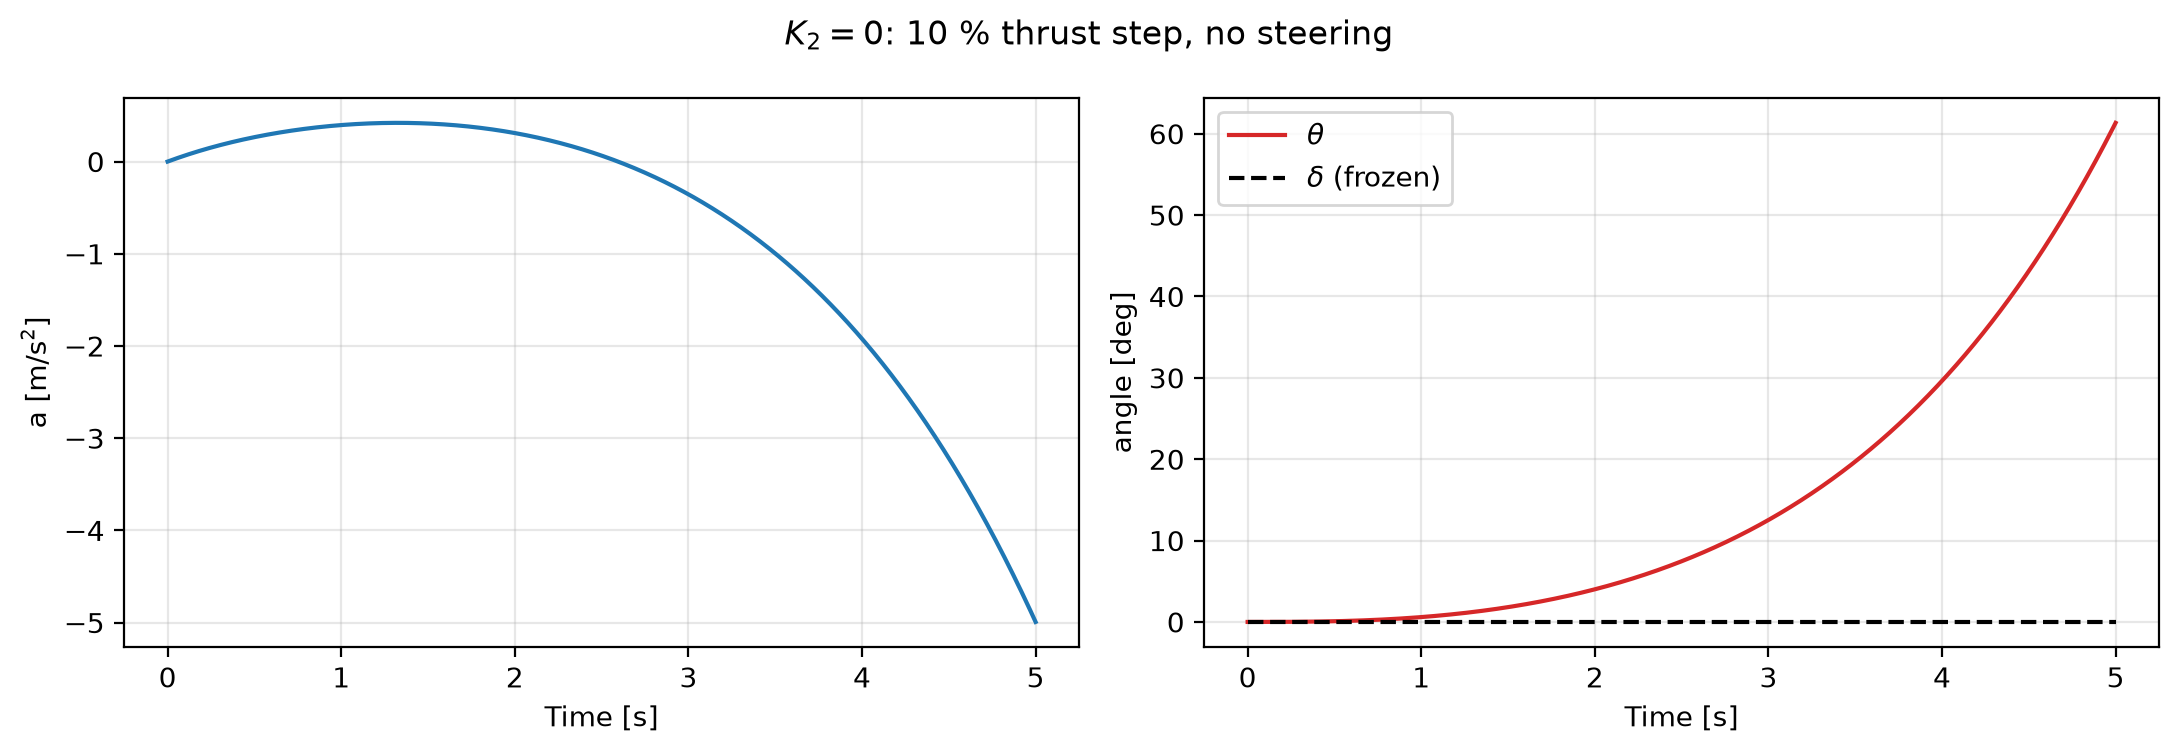
\includegraphics[width=\columnwidth]{imgs/fig_k2_0_unstable.png}
\caption{Con $K_2=0$ el cabeceo se dispara (polo inestable en $+0.557$~s$^{-1}$) mientras la tobera queda en $\delta=0$. Entrada: escalón de 10\,\% de empuje.}
\label{fig:k20}
\end{figure}

De este análisis se desprende la principal implicación: un estado no controlable no se puede mover con ninguna ley de control, por más que se ajusten las ganancias. En los dos casos críticos lo que se pierde es justamente la tobera, el único actuador con autoridad real sobre la actitud, y lo que queda, el empuje, llega a la actitud solo por la desalineación, por lo que es demasiado débil para sustituirla. Sin dirección activa, el cohete no se puede controlar. Por eso perder la tobera es la falla más crítica, mientras que perder el control de empuje resulta tolerable, aunque en ese caso aceleración y ángulo quedan ligados en régimen permanente y no se pueden fijar por separado.

\subsection{Secci\'on E.13: rango recomendado de $K_1$ y $K_2$}

A partir de los resultados anteriores se sabe que muchas combinaciones de ganancias son estables, así que el siguiente paso es definir cuáles son ``buenas''. Para ello se fijaron límites medibles, evaluados con escalones realistas ($u_1=10\,\%$ de empuje y $u_2=5^\circ$): sobreimpulso $M_p\le10\,\%$, tiempo de establecimiento $t_s\le3$~s, error final $e_{ss}\le5\,\%$, deflexión de la tobera $\delta_{\max}\le5^\circ$ y ganancia estática positiva. Con estos criterios se probó una cuadrícula de 2400 pares $(K_1,K_2)$; se conservaron los 187 que cumplen todo y, entre ellos, se eligió el de menor acoplamiento. El barrido está en la celda 84 del notebook (funciones \texttt{gain\_metrics} y \texttt{evaluate\_gain\_grid}), los mapas en la celda 85 y la tabla con todos los números del reporte en la celda 96.

Los mapas de la Fig.~\ref{fig:maps} permiten ver el resultado de un vistazo. Se usan mapas de calor con contorno porque hay dos parámetros, que forman los ejes, y un resultado numérico: cada criterio se traza sobre el plano $(K_1,K_2)$ y la línea blanca marca su límite, de manera que la región buena es la intersección de todas (último panel). Así se observa que el criterio más exigente es la tobera, que solo cumplen 683 de los 2400 puntos. Los mapas también muestran cómo actúa cada ganancia: subir $K_2$ hace la respuesta más rápida y amortiguada, pero mueve más la tobera; subir $K_1$, por su parte, reduce el efecto del comando de cabeceo sobre la aceleración, pero aumenta el del empuje sobre el cabeceo. Con todo ello, el rango y el punto recomendados son
\begin{equation*}
K_1\in[4,\,6.5],\qquad K_2\in[1.1,\,1.45],\qquad (K_1,K_2)_{\text{rec}}=(4.5,\ 1.3).
\end{equation*}

\begin{figure*}[!t]
\centering
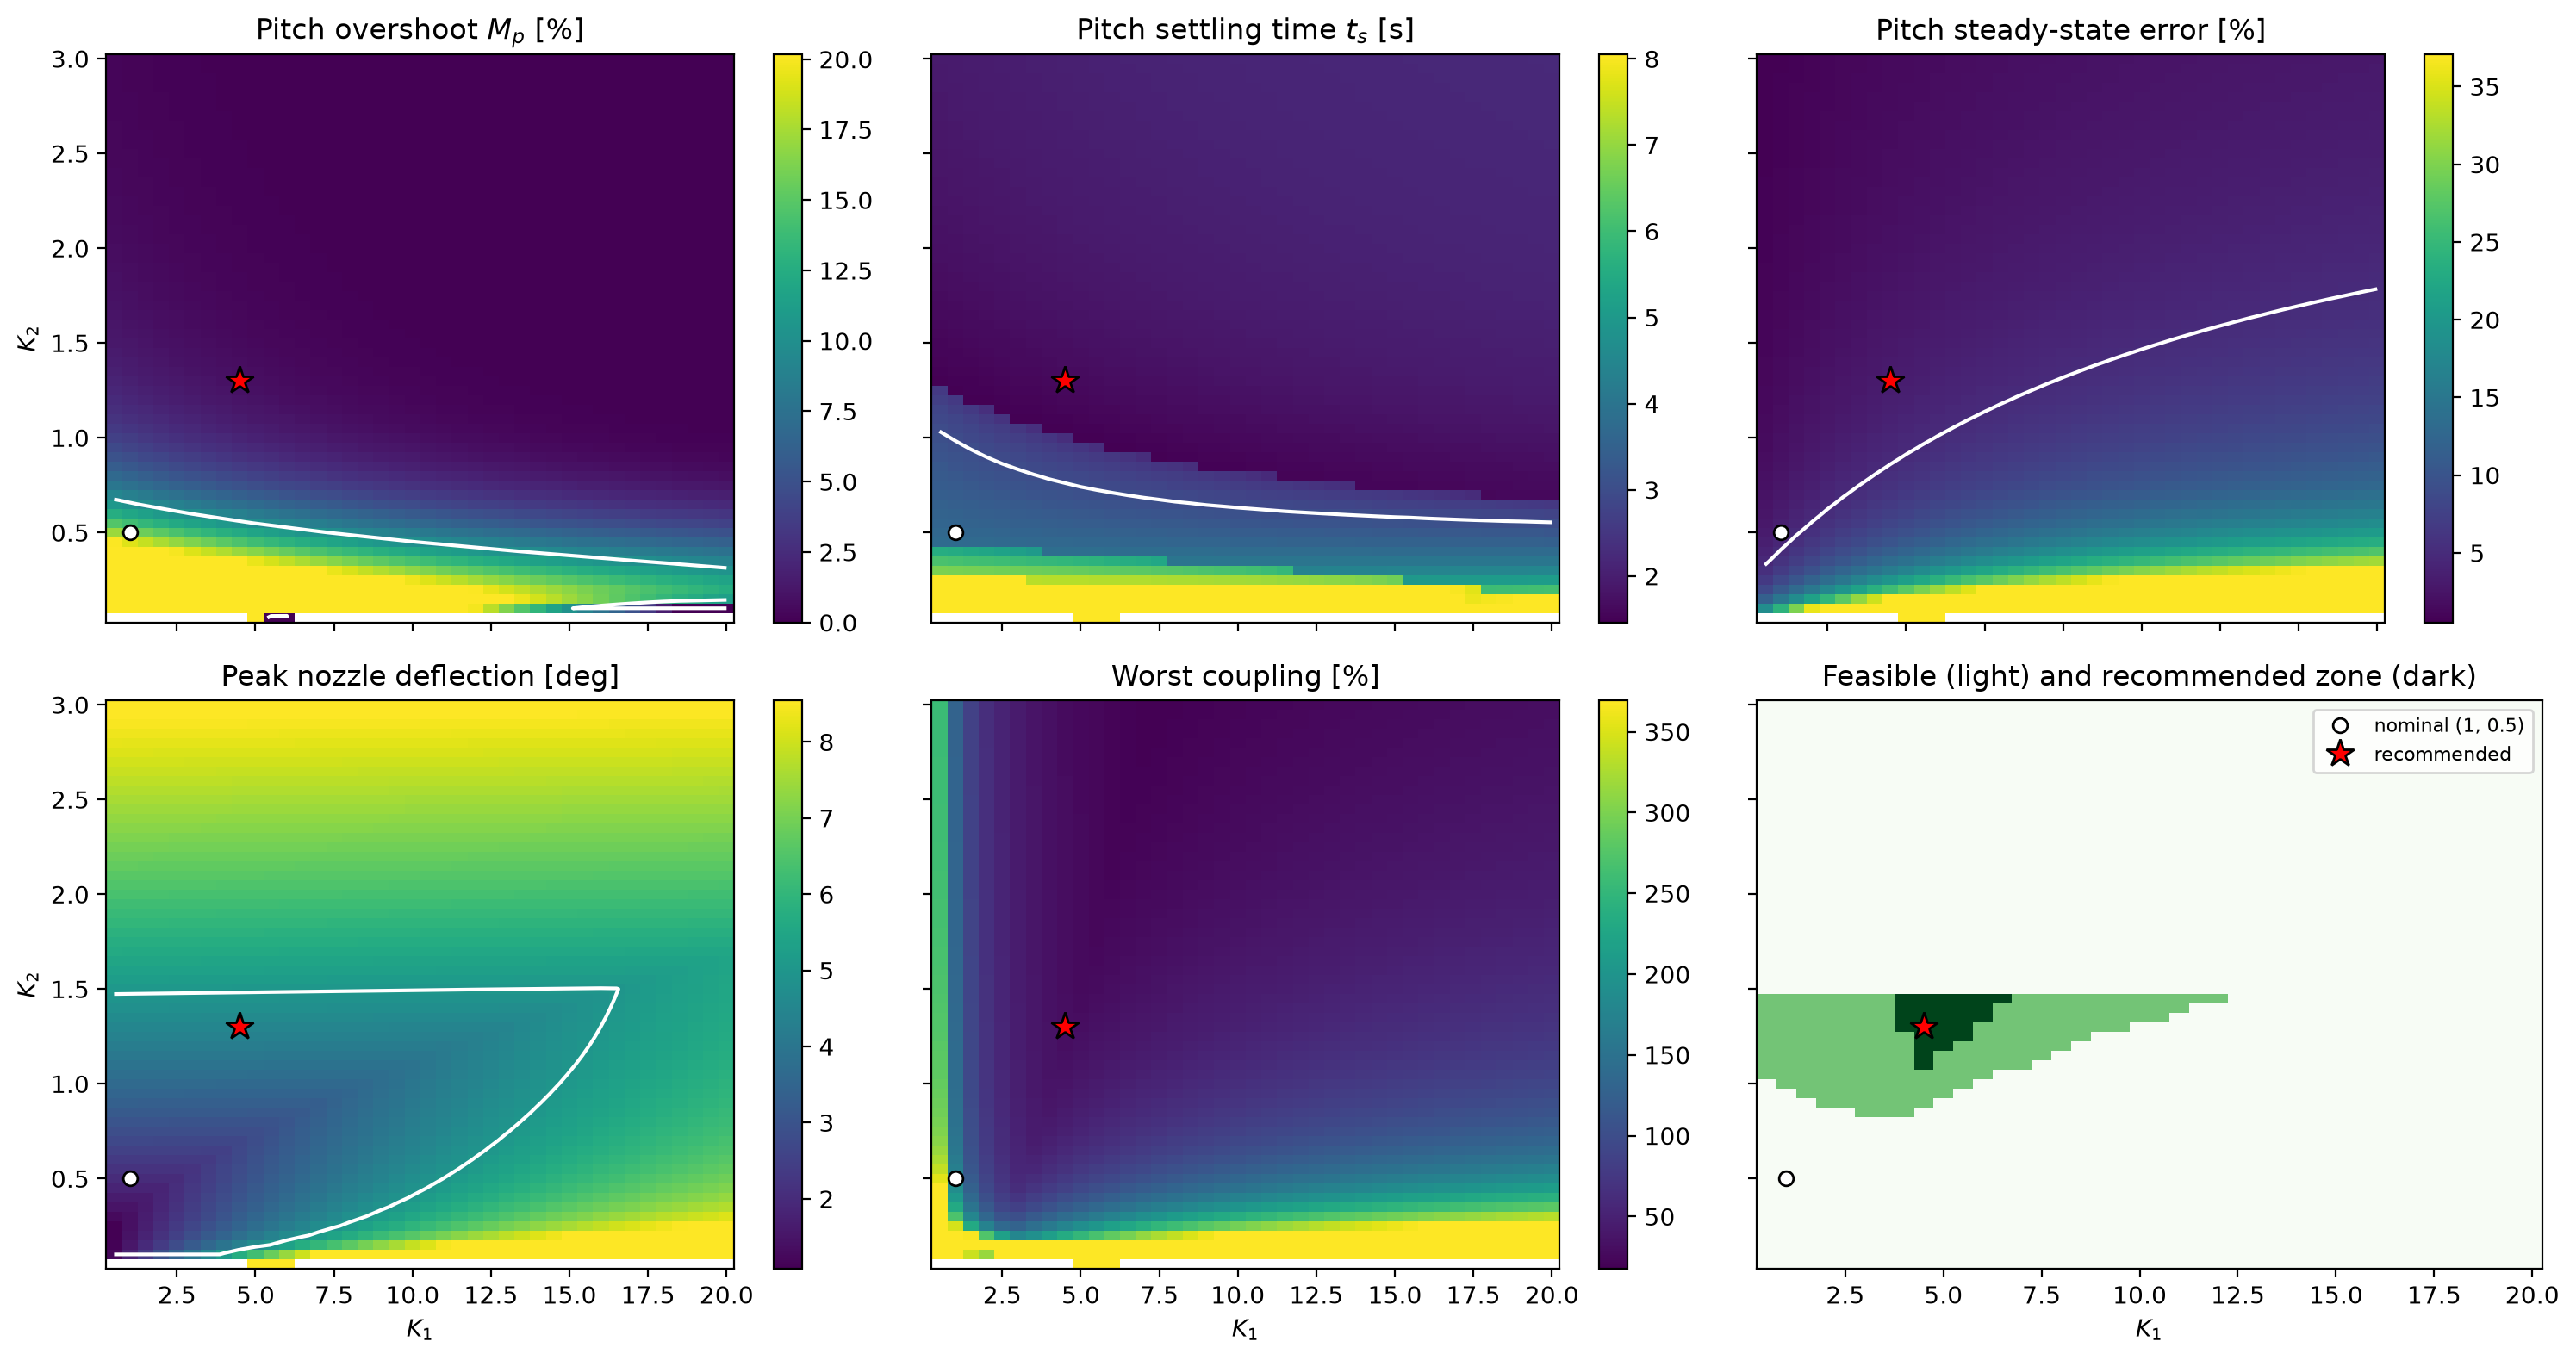
\includegraphics[width=0.85\textwidth]{imgs/fig_metric_maps.png}
\caption{Un mapa por criterio sobre el plano $(K_1,K_2)$; el contorno blanco marca el límite. Último panel: región que cumple todo (verde) y zona recomendada (verde oscuro). Círculo: nominal; estrella: recomendado.}
\label{fig:maps}
\end{figure*}

\begin{table}[H]
\centering
\caption{Comparación de desempeño (celda 96)}
\label{tab:rec}
\resizebox{\columnwidth}{!}{%
\begin{tabular}{|l|c|c|}
\hline
 & Nominal $(1,\,0.5)$ & Recomendado $(4.5,\,1.3)$\\
\hline
Sobreimpulso $M_p$ ($\theta$) & 16.4\,\% & 0.82\,\%\\
Tiempo de establecimiento $t_s$ & 3.64 s & 1.62 s\\
Error final & 4.03\,\% & 3.25\,\%\\
Deflexión máxima de tobera & $2.0^\circ$ & $4.5^\circ$\\
Acoplamiento $u_2\to a$ / $u_1\to\theta$ & 177\,\% / 21\,\% & 31\,\% / 28\,\%\\
\hline
\end{tabular}}
\end{table}

Finalmente, la Tabla~\ref{tab:rec} compara el punto recomendado con el nominal. Las ganancias recomendadas eliminan la oscilación y reducen el tiempo de establecimiento a menos de la mitad, aunque a costa de usar más la tobera ($4.5^\circ$, cerca de su límite de $5^\circ$). Se trata, por lo tanto, de un compromiso en el que nada es gratis. Queda además una limitación: el error final se mide en el cabeceo, y la ganancia estática del canal axial sigue siendo baja (0.21), de modo que la aceleración no sigue exactamente su comando; corregirlo requeriría acción integral.

\subsection{Secci\'on E: efecto del per\'iodo de muestreo $T$}

La propuesta de ganancias debe revisarse también a la luz del muestreo. Un controlador digital mide, calcula y ordena cada $T$ segundos, y entre una medida y la siguiente mantiene la orden constante (retenedor de orden cero, ZOH). Si $T$ es muy grande, el cohete cambia demasiado entre correcciones y el lazo se vuelve inestable, del mismo modo que un auto se saldría del camino si el volante solo se corrigiera una vez por segundo. Como el cómputo también tarda, se modeló además un retardo de una muestra.

Este estudio se encuentra en las celdas 87 a 89 del notebook, con las funciones \texttt{open\_loop\_plant}, \texttt{feedback\_gain}, \texttt{sampled\_loop}, \texttt{spectral\_radius}, \texttt{t\_max} y \texttt{sampled\_step}. Cabe aclarar que no se discretizó la matriz $A$ ya cerrada, porque eso no cambiaría la estabilidad; en su lugar se separaron planta y controlador, y solo se muestreó la realimentación. Como primera verificación (celda 87), el modelo separado reproduce las ecuaciones del enunciado y, cuando $T\to0$, el lazo muestreado tiende al continuo.

Con esta base, la Fig.~\ref{fig:sampstep} superpone las respuestas continua y muestreada: si casi coinciden, $T$ es suficientemente pequeño. Con $T=0.05$~s coinciden incluso con retardo, mientras que con $T=0.1$~s y retardo la respuesta oscila y el sobreimpulso sube a 18.5\,\%. Esto concuerda con la regla práctica de tener entre 10 y 20 muestras dentro del tiempo de subida, ya que con $T=0.05$~s hay 19 (subida de 0.97~s).

\begin{figure}[H]
\centering
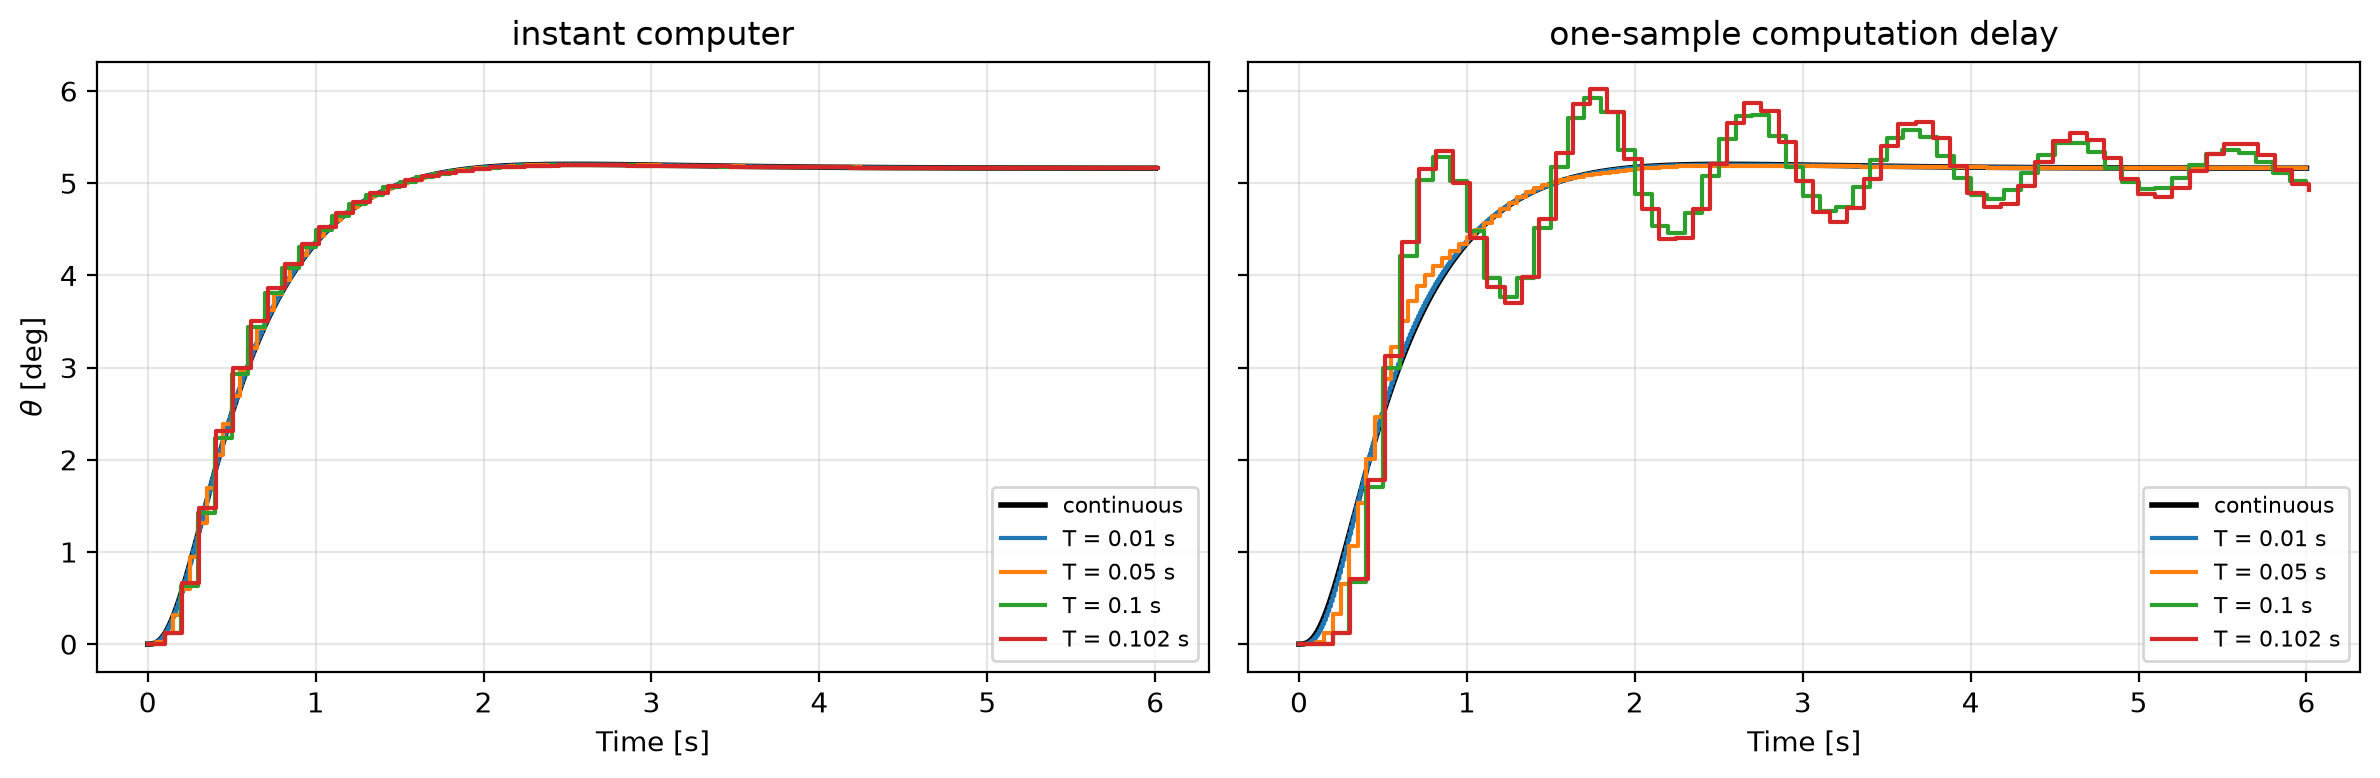
\includegraphics[width=\columnwidth]{imgs/fig_sampling.png}
\caption{Respuesta al escalón de cabeceo ($5^\circ$) con las ganancias recomendadas: lazo continuo frente a muestreado, sin retardo (izquierda) y con retardo de una muestra (derecha).}
\label{fig:sampstep}
\end{figure}

Para encontrar el límite exacto, la Fig.~\ref{fig:samp} grafica contra $T$ el radio espectral, es decir, el mayor ``tamaño'' (módulo) de los autovalores del sistema discreto. La línea en 1 separa los dos comportamientos: por debajo el lazo es estable y por encima, inestable, de modo que el punto de cruce es $T_{\max}$, resumido en la Tabla~\ref{tab:tmax}.

\begin{figure}[H]
\centering
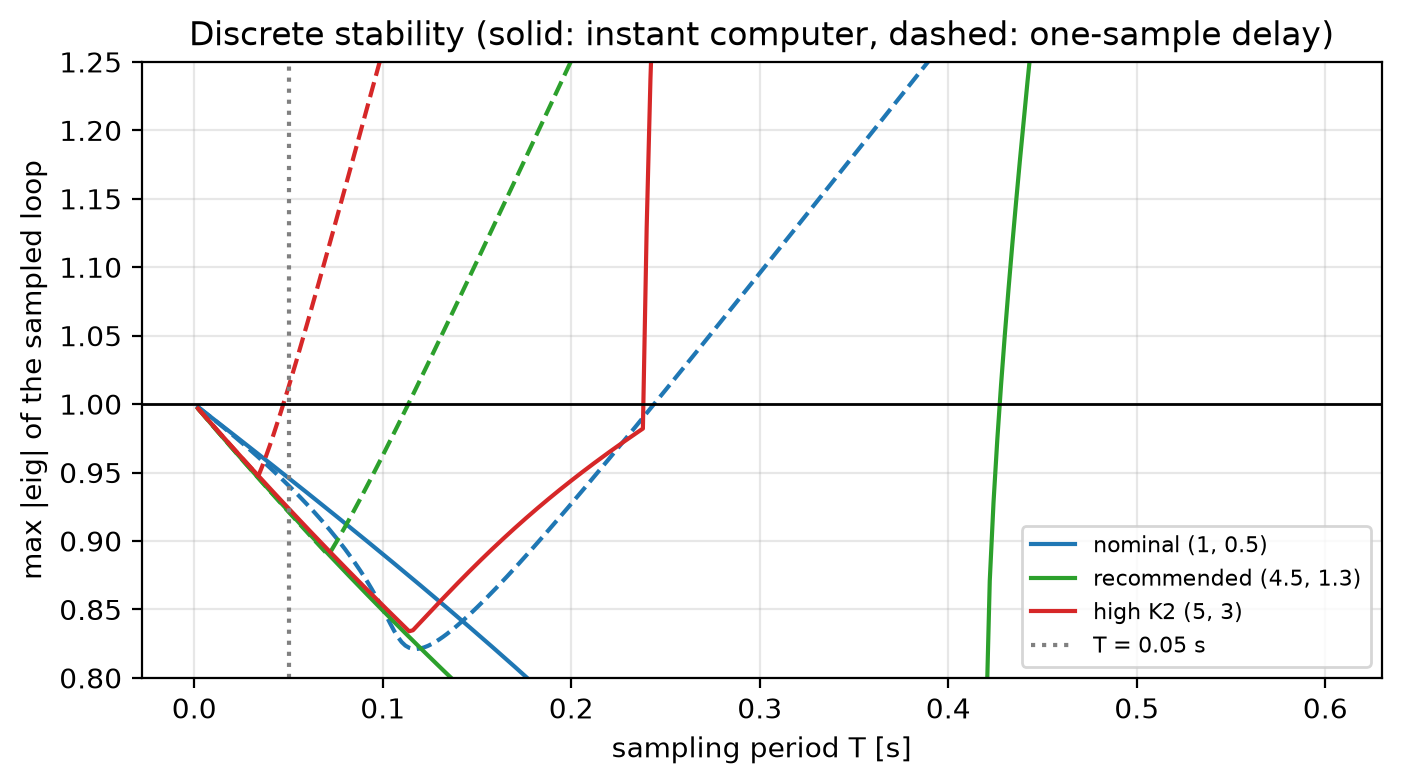
\includegraphics[width=\columnwidth]{imgs/fig_sampling_stability.png}
\caption{Radio espectral frente a $T$ (continua: cálculo instantáneo; discontinua: retardo de una muestra). El cruce con 1 marca $T_{\max}$.}
\label{fig:samp}
\end{figure}

\begin{table}[H]
\centering
\caption{$T_{\max}$ (celda 87)}
\label{tab:tmax}
\resizebox{\columnwidth}{!}{%
\begin{tabular}{|l|c|c|}
\hline
Ganancias & $T_{\max}$ sin retardo & $T_{\max}$ con 1 muestra de retardo\\
\hline
Nominal $(1,\,0.5)$ & 0.999 s & 0.244 s\\
Recomendado $(4.5,\,1.3)$ & 0.427 s & 0.114 s\\
$K_2$ alto $(5,\,3)$ & 0.239 s & 0.047 s\\
\hline
\end{tabular}}
\end{table}

Por último, la Fig.~\ref{fig:tmaxk2} muestra cómo cambia $T_{\max}$ con $K_2$. Las ganancias más altas permiten un $T$ menor, porque el lazo se vuelve más ``nervioso'', y el retardo reduce $T_{\max}$ a menos de un tercio; en cambio, $K_1$ casi no influye, ya que las curvas de $K_1=1$ y $K_1=5$ se superponen. Con $T=0.05$~s queda un margen de 4.9 veces con las ganancias nominales y de 2.3 veces con las recomendadas, pero el caso $(5,\,3)$ ya queda por debajo del margen (0.9 veces). En consecuencia, no conviene subir $K_2$ indefinidamente, porque lo limitan tanto la tobera como el muestreo.

\begin{figure}[H]
\centering
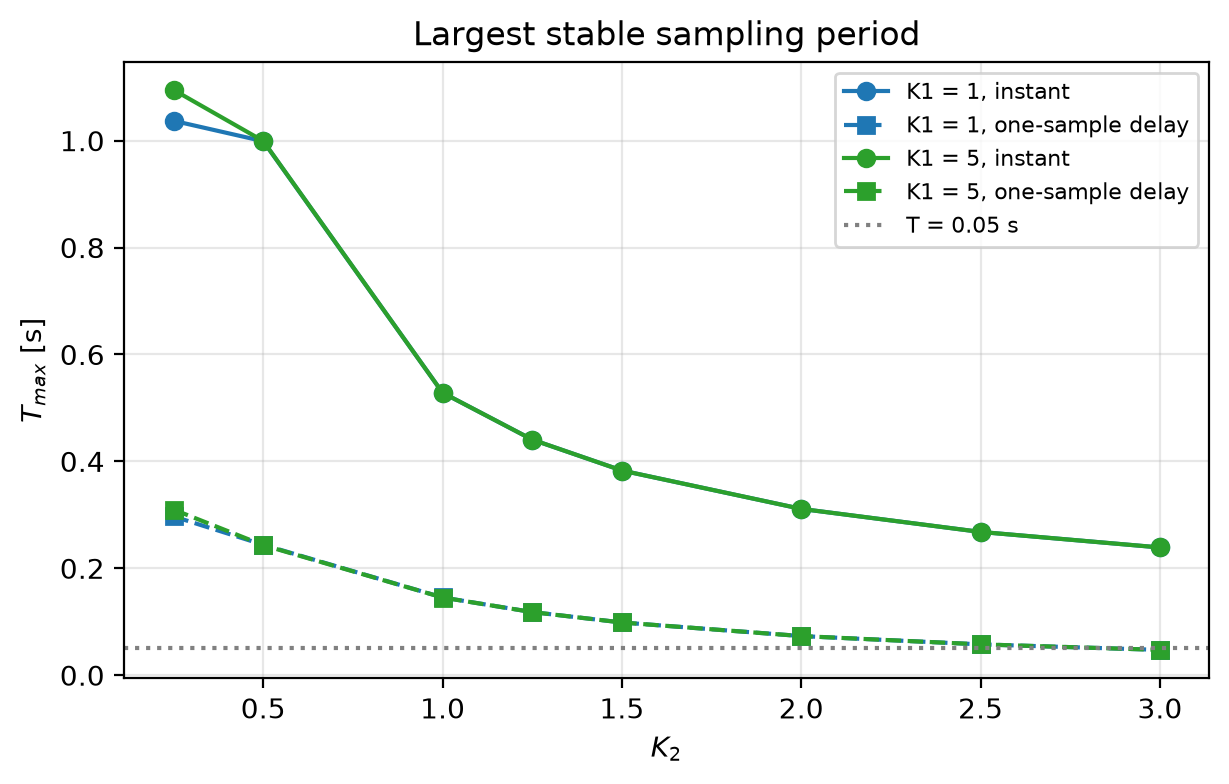
\includegraphics[width=\columnwidth]{imgs/fig_tmax_vs_k2.png}
\caption{$T_{\max}$ en función de $K_2$ para $K_1=1$ y $K_1=5$, sin retardo (círculos) y con retardo de una muestra (cuadrados). Línea punteada: $T=0.05$~s.}
\label{fig:tmaxk2}
\end{figure}

%DISCUSIÓN 
%Esta sección incluye la interpretación de los resultados presentados anteriormente. Se debe incluir la explicación, analisis y comparación entre lo que ya se conoce de literatura anterior y los resultados obtenidos. También  en esta sección se deben responder las preguntas propuestas en la introducción y como se prueba o rechaza la hipotesis propuesta.
\section{Discusi\'on}
\lipsum[1-2]

%CONCLUSIÓN
%Esta sección es un resumen de lo aprendido al final de haber desarrollado el proyecto. Es una sintesís de los resultados más importantes y de lo aprendido de la teoría y la práctica.
\section{Conclusi\'on}
\lipsum[1-1]

%FORMATO APA
\begin{thebibliography}{1}

\bibitem{LabWrite}
M.~Carter, E.~Weiebe, and M.~Ferzli, \emph{LabWrite}, \url{https://www.ncsu.edu/labwrite/index_labwrite.htm}, NC~State~University, 2004.

\bibitem{Fullerton}
D.~Fullerton, \emph{APlusPhysics}, \url{http://www.aplusphysics.com/courses/regents/lab_report.html}, 2016.

\bibitem{Svoronos}
T.~Svoronos, \emph{How I Will Write My Dissertation}, \url{http://teddysvoronos.com/2014/12/26/how-i-will-write-my-dissertation-3/}, 2014.

\bibitem{Clarion}
G. Clarion, \emph{Rocklin High School}, 2009.

\end{thebibliography}

\end{document}


